\documentclass[a4paper,10pt]{scrbook}

\usepackage{geometry}
\geometry{verbose,a4paper,tmargin=2.5cm,bmargin=2.5cm,lmargin=2.5cm,rmargin=2cm}

\usepackage[pdftex]{graphicx}

%\usepackage{ifthen}



% Macht beim fett schreiben auch das Mathe-Zeug fett
%
\newcommand{\allbf}[1]{\textbf{\boldmath#1\unboldmath}}

% FANCY CAPTION
% \caption[#1]{\textbf{#1}#1}
\newcommand{\mycaption}[2]{\caption[#1]{\textbf{\boldmath#1\unboldmath} #2}}







%%%
%%% Now you can use \ifcolor as follows
%%% \ifcolor
%%%    Text parsed by PDFLaTeX
%%% \else
%%%    Text parsed if PDFLaTeX is not used
%%% \fi
%%% 
\newif\ifcolor\colortrue



%
%   COLOR
%
%
\usepackage{color}
\definecolor{brightred}{rgb}{1,0.9,0.9}
\definecolor{brightgreen}{rgb}{0.9,1,0.9}
\definecolor{brightblue}{rgb}{0.9,0.9,1}
\definecolor{brightyellow}{rgb}{1,1,0.85}

\definecolor{lightred}{rgb}{1,0.75,0.75}
\definecolor{lightgreen}{rgb}{0.75,1,0.75}
\definecolor{lightblue}{rgb}{0.75,0.75,1}
\definecolor{lightyellow}{rgb}{1,1,0.75}

\definecolor{red}{rgb}{1,0,0}
\definecolor{green}{rgb}{0,1,0}
\definecolor{blue}{rgb}{0,0,1}

\definecolor{darkred}{rgb}{.7,0,0}
\definecolor{darkgreen}{rgb}{0,.7,0}
\definecolor{darkblue}{rgb}{0,0,.7}

\definecolor{white}{rgb}{1,1,1}
\definecolor{lightgray}{rgb}{0.95,0.95,0.95}
\definecolor{gray}{rgb}{0.5,0.5,0.5}
\definecolor{black}{rgb}{0,0,0}

\definecolor{marker}{rgb}{0.9,0.9,0.9}
\definecolor{urgent}{rgb}{1,0,0}
\definecolor{discreeturgent}{rgb}{1,0.5,0.5}
\definecolor{discreetcomment}{rgb}{0.25,0.9,0.25}
\definecolor{checked}{rgb}{0,.7,0}



%\newif\ifshowtasks\showtaskstrue
\newif\ifshowtasks\showtaskstrue
\newcommand{\task}[1]{\ifshowtasks\textcolor{discreeturgent}{~#1~}\else\fi}
\newcommand{\comment}[1]{\ifshowtasks\textcolor{discreetcomment}{~#1~}\else\fi}
\newcommand{\drain}[1]{}

%
%    LISTINGS
% \begin{lstlisting}[float,caption=A floating example]
%    for i:=maxint to 0 do
%    begin
%      { do nothing }
%    end;
%    Write(’Case insensitive ’);
%    WritE(’Pascal keywords.’);
% \end{lstlisting}
%
% for referencing line numbers use (*@\label{comment}@*)  inside the lstlistings enviroment
\usepackage{listings}
\ifcolor
          \lstset{							% general command to set parameter(s)
               escapeinside={(*@}{@*)},
               xrightmargin=0.5cm,					% for centering
               xleftmargin=1.5cm,					% .. \textwidth shrinks after the first time, which is stupid
               framexleftmargin=20pt,					% for having the numbers beneath the h rules
               framexrightmargin=0pt,
               framextopmargin=2ex,					% draw good looking space between the lines
               framexbottommargin=2ex,					%... and the listing
               frame=single,						% h rules top and bottom
               language=C,
               tabsize=4,
               numbers=left,
               numberstyle=\footnotesize, 
               numbersep=8pt,
               basicstyle=\ttfamily\scriptsize, 		% print whole listing small
               breaklines=true,
               keywordstyle=\color{black}\bfseries,		% underlined bold black keywords
               identifierstyle=,				% nothing happens
               commentstyle=\color{darkblue}\itshape,		% white comments
               stringstyle=\ttfamily, 				% typewriter type for strings
               morekeywords=[2]{and,or,not},
               emph={wichtiges,zeug},				% additional keywords
               emphstyle=\underbar,
               showstringspaces=false} 				% no special string spaces
\else
          \lstset{						% general command to set parameter(s)
               escapeinside={(*@}{@*)},
               xrightmargin=0.5cm,				% for centering
               xleftmargin=1.5cm,
               framexleftmargin=20pt,				% for having the numbers beneath the h rules
               framexrightmargin=0pt,
               framextopmargin=2ex,				% draw good looking space between the lines
               framexbottommargin=2ex,				%... and the listing
               frame=single,					% h rules top and bottom
               language=C,
               tabsize=4,
               numbers=left,
               numberstyle=\footnotesize, 
               numbersep=8pt,
               basicstyle=\scriptsize\ttfamily,			% print whole listing small
               breaklines=true,
               keywordstyle=\color{black}\bfseries,		% underlined bold black keywords
               identifierstyle=,									% nothing happens
               commentstyle=\color{black}\itshape,			% white comments
               stringstyle=\ttfamily, 							% typewriter type for strings
               morekeywords=[2]{and,or,not},
               emph={wichtiges,zeug},								% additional keywords
               emphstyle=\underbar,
               showstringspaces=false} 						% no special string spaces
\fi

%
\usepackage[labelfont={bf},font=small]{caption,subfig} 
% justification=raggedright,format=hang,labelfont={bf},font=small
% justification=justified,singlelinecheck=false

%
%    HYPERREF
%
%    (depends on z_layout_settings color)
%
% NO HANDLING YET FOR NOT PDF!!!
\ifcolor
  \usepackage[pdftex,
            colorlinks=true, linkcolor=blue, urlcolor=blue, citecolor=blue,
            raiselinks=true,
            bookmarks=false,
            bookmarksopenlevel=1,
            bookmarksopen=true,
            bookmarksnumbered=true,
            hyperindex=true,
            plainpages=false,% correct hyperlinks
            pdfpagelabels=true%,% view TeX pagenumber in PDF reader
            %pdfborder={0 0 0.5}
            ]{hyperref} % erzeuge Hyperlinks z.B. für pdflatex
\else
  \usepackage[pdftex,
            colorlinks=true, linkcolor=black, urlcolor=black, citecolor=black,
            raiselinks=true,
            bookmarks=false,
            bookmarksopenlevel=1,
            bookmarksopen=true,
            bookmarksnumbered=true,
            hyperindex=true,
            plainpages=false,% correct hyperlinks
            pdfpagelabels=true%,% view TeX pagenumber in PDF reader
            %pdfborder={0 0 0.5}
            ]{hyperref} % erzeuge Hyperlinks z.B. für pdflatex
\fi





\newcommand{\lstsetCPP}{%
\ifcolor%
\lstset{
	escapeinside={//(@*}{*@)},
	language=C++,
	frame=single,
	numbers=left,
	backgroundcolor=\color{brightblue}
	}%
\else%
\lstset{
	escapeinside={//(@*}{*@)},
	language=C++,
	frame=single,
	numbers=none,
	backgroundcolor=\color{white}
	}%
\fi%
}

\newcommand{\lstsetARCHEDXML}{%
\lstset{
	escapeinside={<!--(@*}{*@)-->},
	language=XML,
	frame=single,
	numbers=left,
	backgroundcolor=\color{lightyellow}
	}%
}

\newcommand{\lstsetJUSTXML}{%
\lstset{
	escapeinside={<!--(@*}{*@)-->},  % <!--(*@\label{comment}@*)-->
	language=XML,
	frame=single,
	numbers=left,
	backgroundcolor=\color{brightyellow}
	}%
}


\newcommand{\lstsetKSH}{%
\lstset{
	escapeinside={(@*}{*@)},
	language=ksh,
	frame=single,
	numbers=none,
	backgroundcolor=\color{lightgray}
	}%
}

% Sometimes latex just won't accept a line break.
% With this command you can do it anyway! HAR HAR HAR
\newcommand{\forcelinebreak}{
%\vspace{\bigskipamount}
\hspace*{\fill} \\
} 


\usepackage{framed}                                %for shaded and framed paragraphs
\usepackage{textcomp}                              %for various symbols, e.g. Registered Mark
%
\def\efill{\hfill\nopagebreak}%
\hyphenation{Nordu-Grid}
\setlength{\parindent}{0cm}
\setlength{\FrameRule}{1pt}
\setlength{\FrameSep}{8pt}
\addtolength{\parskip}{5pt}
\renewcommand{\thefootnote}{\fnsymbol{footnote}}
\renewcommand{\arraystretch}{1.3}
\newcommand{\dothis}{\colorbox{shadecolor}}
\newcommand{\globus}{Globus Toolkit\textsuperscript{\textregistered}~2~}
\newcommand{\GT}{Globus Toolkit\textsuperscript{\textregistered}}
\newcommand{\ngdl}{\url{http://ftp.nordugrid.org/download}~}
\definecolor{shadecolor}{rgb}{1,1,0.6}
\definecolor{salmon}{rgb}{1,0.9,1}
\definecolor{bordeaux}{rgb}{0.75,0.,0.}
\definecolor{cyan}{rgb}{0,1,1}
%
%----- DON'T CHANGE HEADER MATTER

\hypersetup{
  pdfauthor = {},
  pdftitle = {Webservices},
  pdfsubject = {Paper subject},
  pdfkeywords = {HED,ARC},
  pdfcreator = {PDFLaTeX with hyperref package},
  pdfproducer = {PDFLaTeX}
}

\begin{document}

% Conventions:
% * Web Service
% * server configuration file (arched -c server_configuration_file.xml)
% * client configuration file (loaded by the client in the same manner like arched does)
% * Abbreviation of protocols are written with big letters (IP TCP TLS HTTP,...)

\def\today{\number\day/\number\month/\number\year}

\begin{titlepage}

\begin{tabular}{rl}
\resizebox*{3cm}{!}{
\includegraphics{images/ng-logo.png}}
&\parbox[b]{2cm}{\textbf \it {\hspace*{-1.5cm}NORDUGRID\vspace*{0.5cm}}}
\end{tabular}

\hrulefill

{\raggedleft NORDUGRID-TECH-19\par}

{\raggedleft \today\par}

\vspace*{2cm}

%%%%---- The title ----
{\centering \textsc{\Large Webservice programming Tutorial}
\\\vspace{1cm} \normalsize\textcolor{discreeturgent}{I am currently working on this document, but I appreciate all comments and suggestions. \\e-mail: glodek@inb.uni-luebeck.de} % DELETE ONLY THAT LINE!!!
\Large \par}
\vspace*{0.5cm}

%%%%---- A subtitle, if necessary ----
%{\centering \textit{\large Paper subtitle}\large \par}

\vspace*{1.5cm}
%%%%---- A list of authors ----
    {\centering \large Michael Glodek, Steffen M\"oller, ... \large \par}

%%%%---- An abstract - if style is article ----
%\begin{abstract}
%The abstract
%\end{abstract}
\end{titlepage}

\tableofcontents                          %Comment if use article style
\newpage
%\chapter{Preface}
%\section{Introduction}                    %Use Sections for articles
%\label{sec:intro}

\sloppy

\chapter{Introduction}

This document gently introduces to the preparation of standalone Web Services and cognated clients with the Advance Resource Connector (ARC).
The reader is guided through a series of practically oriented examples.
Each is accompanied by explanations of the main concepts of the software architecture.
No particular skills are required to follow the presented steps.
It is however beneficial to have some basic comprehension of the programming language C++, the file format XML and any regular UNIX shell.
To start, the user shall have an installation of ARC-1, as it is performed with current RPM or .deb packages\footnote{see http://wiki.nordugrid.org for explicit instructions for setup}.\\


The ARC server provides access to services.
These are executed on the same machine that the server is installed on.
Some services, like the A-REX service, will delegate computational efforts to other machines
via additional software like a local queueing system.
But the A-REX service itself does not migrate away to other machines - at least this
has not been implemented yet.
Services may comprise computational tasks (e.g., some secret and strongly
patented algorithm), allow arbitrary computations (like ARC's A-REX or
Amazon's clouds) or provide access to other resources like a particular
database or to arbitrary disk space (like ARC's hopi or bartender).\\


Services are invoked using software programs, which are referred to as clients. 
These programs may directly perform the interactions of human users or request a performance of other services of another server (here the first service is in the role of a client, too).
The tasks of servers and clients are well defined. If servers are not busy reacting to a client's request, then they are waiting. The task of servers can be subdivided into:
\begin{itemize}
 \item Wait for client request
 \item Receive the request
 \item Perform the desired service
 \item Create a response for the client
 \item Send response to the client
 \item Wait for next client request
\end{itemize}
While the server waits passively for a request, the client acts actively:
\begin{itemize}
 \item Create a request
 \item Transmit the request to the server which provides the desired service.
 \item Wait for the reply
 \item Receive the response from the server.
 \end{itemize}
Servers provide access to a single or a set of services. In ARC services are provided by the Hosting Environment Demon (HED) which enables the installation of several services on one network access point. 
\forcelinebreak

In general, the implementation of a client is easier than the implementation of the server. 
ARC is designed as a middleware which encapsulates typical challenges of server-client infrastructures (security, exception handling, extensibility) and abstracts from the underlying computer architecture (heterogeneity of computers, computer location, protocols).
The core of ARC is the prior mentioned HED (Hosting Environment Daemon).
To the administrator HED is mostly visible as the single binary that is started and configured by a file that describes services' that shall be prepared by HED. 
Conceptionally, the HED determines how services shall be organised both as a principle, and for any given ARC-run server.
HED determines the very explicit presence or absence of a service at a particular address. Its many configurable layers are described later in this tutorial. 
%
At the time of writing, the endpoint of the HED will be a SOAP based  Web Service.
SOAP is a long established XML-based standard for Web Service communication.
ARC abstracts from this format, but nevertheless it is useful to be aware of
the underlying message transport mechanism.

%which implicate several advantages.
%The XML file format is not restricted to a certain set of tags but can be expanded in such a way as to fit almost any kind of service. It is not a proprietary format and as a result many libraries in almost any language are capable in creating that kind of format.Likewise, XML is also suitable for the usage between heterogeneous platforms.However, while the client can be implemented very straight, the service has to fit a certain layout.In the present guide four kinds of webservices will be introduced: a simple time service, an echo service, a secure echo service and a service with a persistence state .\\


 


\section{Hosting Environment Daemon}

The HED which was already mentioned in the section above is an essential part of the ARC middleware. 
Its task is to provide the hosting of various services at the application level and is based on the idea modularity. % allows its dynamic extension.
The HED consists of components called Message Chain Components (MCC), Plexer, Services, and several modules, which shall aid the programmer to simplify the development of the Web Services: Config, Loader, Logging, XMLNode et cetera.
The MCCs are ordered within a layered structure. 
Each MCC provides a certain functionality such as communication between two applications (MCC TCP), secure data transfer (MCC TLS) or client-server architecture (MCC HTTP).
Figure~\ref{fig:HED_internal} illustrates a typical setup of a server-sided HED.

\begin{figure}[htb]
	\centering
	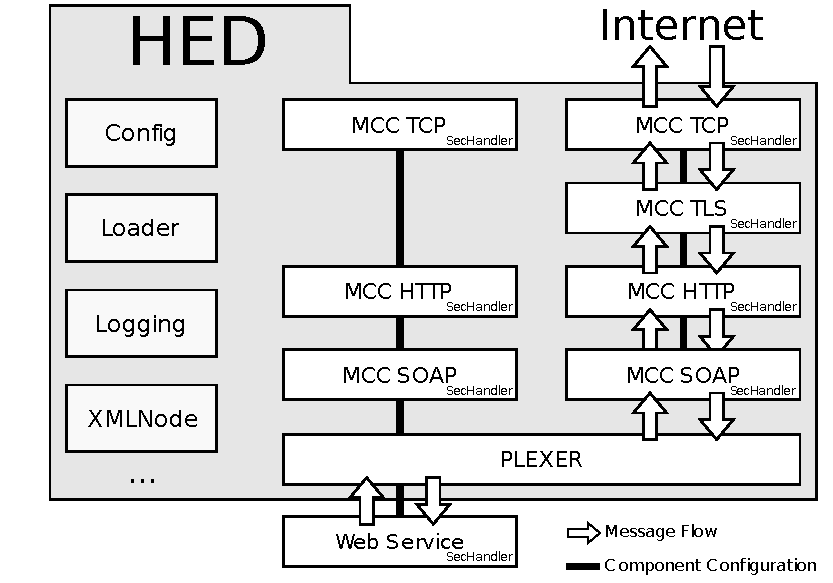
\includegraphics[width=13cm]{tex_introduction/HED2.pdf}
	\mycaption{Example of a HED structure providing a Web Service}{The HED consists of several layers which are connected with each other. The arrow indicate the message flow of the used configuration. The MCCs and Services may hold a SecHandler in order to give additional security. Additional modules (on the left) are used within the HED. \task{Why is the Web Service in all images outside of the HED?} } % TODO: Reverse order of layers, s.t. the highest layers are above and the lowest layer are at the bottom
\label{fig:HED_internal}
\end{figure}

The MCCs are connected which each other and passing incoming and outgoing message to the upper or the respective lower layer. In case of outgoing messages a MCC is wrapping the data of the upper layer as a payload into their own protocol (while incomming message will be unwrapped).
The lowest layer has to be a transport protocol like TCP which enables the transmission between two applications.
Technically there are even lower layers required needed for the communication but they are already realised within the operating system and the  network card.
TCP is well suited for the application because it provides a reliable and ordered delivery of a byte stream.
Above the TCP layer is the Hypertext Transfer Protocol (HTTP). 
In case a security layer is desired (i.e. for authentication), the TLS (Transport Layer Security formerly known as SSL, Secure Sockets Layer) has to be inserted between the TCP and HTTP layers.
The HTTP provides the client-server architecture. It is stateless but offers several extensions for requests, header information and status codes. Furthermore HTTP enables the usage of Uniform Resource Locators (URL) which is used by ARC to multiplex between different services. The multiplexing layer can also be defined within the HED and is called Plexer.
Depending on the path of the URL the Plexer passes messages to a defined SOAP service which again passes the message to the Web Service~\cite{QIANG_2005}.\\
% QUESTION: Why is the plexer always illustrated  being above the SOAP MCC. There's no config file example like that in the tree.
%In my understanding (because plexer is not my initial idea), plexer (as a sort of hub) can be put at both after http or soap. If you put after soap,then you are doing switching for different web services. While I put it after http, because somehow, I need to switch the message after http-processing, in more detail, one branch for soap and then web service/s, one branch for a non-soap service/server (the SP Service is not a service based on SOAP, actually it is based on http, so it is kind of web application).


The structure of the HED can be configured freely by modifying the server configuration file.
A first impression how the HED can be configured shall be given in the following example which corresponds to the HED shown in Figure~\ref{fig:HED_internal}.
It uses the ARC echo service that is shipped for testing purposes with the ARC source code.



\subsection{The ARC Echo Web Service}
\label{sec:arc_echo_web_service}


The first example shall give a basic understanding in how to configure the HED for setting up a novel service.
The task is to setup the regular ARC Echo Web Service.
On the command line, all that needs to be done is to invoke the \textit{arched} daemon with a suitable server configuration file.
Such a fitting server configuration file is shown in Listing~\ref{lst:arched_arcecho_xml}.
It is written in XML. Its structure is based on the XSD schema listed in~\ref{sec:impXSD} in Listing~\ref{lst:mcc.xsd}.\\ 

\lstsetARCHEDXML
\lstinputlisting
	[label=lst:arched_arcecho_xml,float=htb,
	caption={[HED configuration file.]
	\textbf{HED configuration file.}}]
{../examples/src/services/arched_arcecho.xml}
The first line of the XML file contains the XML declaration.
Several attributes can be defined here but at least the XML version should be specified.
The configuration as a whole is encapsulated by the element \textit{ArcConfig}. It also performs the setting of namespaces, which are expected to be mostly invariant across all server installations. % ABBREVIATIONS?? - MG
The \textit{Server} element, to be found at line~\ref{lst_code:arched_arcecho_Server}, provides basic settings for the daemon such as the location of the Pid-file or ofthe Log-file.
The \textit{ModuleManager} holds the \textit{path} to the plugin libraries.
Several paths may be defined here.
Due to the fact that the first library matching the plugin name is loaded, the order is relevant.
The path should be at least assigned to the ARC installation directory.
Otherwise, the set of ARC MCC plugins might not be found.
The next elements are holding the name of the plugins to be loaded (line~\ref{lst_code:arched_arcecho_Plugins}).
The names have to correspond to the names of the dynamic libraries within the path defined in the \textit{ModuleManager}.
Finally, the chain, which creates the layered structure, is declared within the element \textit{Chain}.
It is composed of the elements \textit{Component}, \textit{Plexer} and \textit{Service}.
Due to a MCC plugin may contain several components, one has to specify more exact which one to load. This is to be done using the \textit{name} attribute i.e. the plugin \textit{mcchttp} realises two components: \textit{http.service} and \textit{http.client}. Since we are defining a configuration file for a service, the \textit{http.service} should be used.
Furthermore the elements may have the attribute \textit{id} as a unique identifier within the file.
Regarding the components and the services a plugin (implemented as a *.so file that is searched in the paths previously specified) has to be loaded which provides the implementation of its functionality. The further configuration depends on the plugin's individual functionality.\\
%
% within the chain ... 3 types of elements
%
%Its needed to distinguish between the plugins and the components.
%The plugins refer to shared libraries that can be integrated as modules with the HED to extend its functionality.
%The Components refer to the implementation of Web Services within any of those libraries.


A \textit{Chain} will determine the path that an event takes to be noticed.
The first component of the chain is the \textit{tcp.service}.
As to be seen, the port 60000 is assigned to the server to listen to.
The port can be an arbitrary number.
However, the number 60000 is commonly used for a HED providing the A-REX Web Service (the one organising the computation on a site) and the number 50000 is found commonly used for a HED running Web Services for storage.
This way, one can organise a single server to offer multiple HED instances.
The stream which is received by this component is passed to the component defined by the \textit{next} attribute.
In the present case, it will be passed to the component with the \textit{id} attribute named \textit{http}.
In this way, the message is be passed to higher layers until it reaches the \textit{Plexer}.
Depending on the path of the URL which was demanded by the HTTP, the Plexer multiplexes the request to the right Web Service\task{, the right function to execute according to the component IDs and plugin names. -- ??MG}
The plexer will thus allow to have multiple Web Service listen to the same port.
The path, declared within the \textit{next} attribute, corresponds to a regular expression and leads to the service with the id named \textit{echo}. 
Hence, the service will now be reachable under URL \textit{http://localhost:60000/echo}.
It will finally process the message and create a new message which will be returned all the way back to the TCP component.
The Echo Web Service itself is provided by the ARC package.
Additional invariant parameters are passed by the elements \textit{prefix} and \textit{suffix}.
They set the characters which will enclose the echoed string.
\task{The images of the HED structure always are ordered like: TCP - TLS - HTTP - PLEXER - SOAP - Web Service   but the source code examples are: TCP - TLS - HTTP - SOAP - PLEXER - Web Service}

To create the daemon corresponding to the defined server configuration file, ARC provides the program called \textit{arched}.
The manner of invokation is to been seen in Listing~\ref{lst:arcecho_arched_invokation}.
\lstsetKSH
\begin{lstlisting}[
label=lst:arcecho_arched_invokation,float=htb,
caption={[Invokation of the arched daemon in order to start the ARC Echo Web Service.]
         \textbf{Invokation of the Arched Daemon.\textcolor{white}{hmf}}}]

$ arched -c arcecho_no_ssl.xml && echo Daemon started || echo Daemon failed
 Daemon started
$
\end{lstlisting}

% $ rm -f /var/log/arched.log
% $ tail -n100 -f /var/log/arched.log
%...
%$ killall arched
%
%
The name of the program is followed by the parameter \textit{-c}.
The string following that argument contains the path to the configuration file.
Once the server is running, the client can be used as described in Listing~\ref{lst:arcecho_client_invokation}.
\lstsetKSH
\begin{lstlisting}[
label=lst:arcecho_client_invokation,float=htb,
caption={[Usage of the ARC Echo client.]
         \textbf{Usage of the Arc echo client.\textcolor{white}{hmf}}}]
$ arcecho http://localhost:60000/Echo text
[ text ]
\end{lstlisting}

In this example, the server and the client are running on the same computer such that the hostname \textit{localhost} can be utilized. 
For debugging it is advisable to check the logfile which was assigned inside the server configuration file.
It is commonly found at /var/log/arched.log.

The following chapters explain how to develop custom Web Services.
The first one will be the simple Time Web Service.













\chapter{The time webservice}


The first implementation of a Web Service will be a simple time service. 
In case that the service receives a request of a client, it will respond with a string containing the system time.
For simplicity the service will not parse the request but always return the current time.
In the following subsections the implementation of the service and the client will be presented. 


\section{Service}

In Arc the services are implementated as plugins such that they can easily be included or excluded by modifiying the HED configuration file as it was to be seen in Listing~\ref{lst:arched_arcecho_xml}.
Listing~\ref{lst:time_arched_cpp} contains the C++ implementation of the time service plugin.
The proper class definition of the object \textit{TimeService} is defined in the corresponding header file which is not shown here. It inherits from an object called \textit{Service} defined in the Arc library.
The key element for each plugin is the struct \textit{PluginDescriptor} named \textit{PLUGINS\_TABLE\_NAME} to be seen in line~\ref{lst_code:time_cpp_ptn}. 
%The struct defines basic entities of the service and provides a pointer to the method which is able to create an instance of the time service plugin.
Within the struct a unique plugin name, the type of the plugin, its version and a pointer to a function which returns the instance of the time service has to be defined.
The function which returns the pointer of the instance is desclared in line~\ref{lst_code:time_cpp_get_service}. 
The interface demands an object \textit{PluginArgument} as a parameter but because we are writing a plugin which inherits from \textit{Service}, we are able to expect the \textit{PluginArgument} to be a \textit{ServicePluginArgument}.
%	In the first line of the service the object is downcasted with the operator dynamic_cast
The \textit{ServicePluginArgument} provides access to the HED configuration and the message chain of the service.
%       operator Config* (void) { return config_; };
%       operator ChainContext*   			an interface to manipulate chains stored in Loader
%
%
%
%
The time service uses the namespace \textit{ArcService}. The constructor can be found in line~\ref{lst_code:time_cpp_constructor} and the deconstructor in line~\ref{lst_code:time_cpp_deconstructor}.%
\lstsetCPP%
\lstinputlisting[
	label=lst:time_arched_cpp,
	caption={[C++ implementation of the time service. Filename: timeservice.cpp]
	\textbf{C++ implementation of the time service. Filename: timeservice.cpp}}
	]%
{../src/services/timeservice/timeservice.cpp}%
In the context of the simple service they don't contribute with any functionality.
The method \textit{process} which is required by the inherited class \textit{Service} is defined in line~\ref{lst_code:time_cpp_process} and realises the desired service. 
The parameters \textit{inmsg} and \textit{outmsg} are references to the incoming and outgoing messages. Furthermore the method \textit{process} returns the object \textit{MCCStatus} which is representing the result of the service achieved. 
Within the method \textit{process}, the service first determines the current time and than creates a SOAP payload using the object \textit{PayloadSOAP} on line~\ref{lst_code:time_cpp_process_payloadSOAP}. 
The object \textit{PayloadSOAP} provides enough functionality to create a XML message which is conform to the SOAP protocol 
(The apperance of the generated request and response will be discussed later on page~\pageref{lst:time_client_request}). 
%
%
In the current case the payload consists of two elements nested into one another. The element \textit{time} holds the element \textit{timeResponse} which again holds the string containing the current time.
Within the line~\ref{lst_code:time_cpp_process_message_payload} the payload is stored in the message. 
In case nothing unexpected happened during the message is processed, the function returns with an \textit{MCCStatus} set to \textit{OK} as to be seen in line~\ref{lst_code:time_cpp_return}.\\


%The service has to be compiled into a dynamic library named \textit{libtimeservice.so}, in order
%To run the service, one has to compile the source code into a dynamic library named \textit{libtimeservice.so}.\\
%After the service is shipped into the library \textit{libtimeservice.so} it needs to be copied into the directory \textit{/tmp/arc/tutorial/lib} so it can be found by the \textit{ModuleManager} of the HED. 

In order to run the service, it has to be compiled into a dynamic library named \textit{libtimeservice.so}.
The library has be to be copied into the directory \textit{/tmp/arc/tutorial/lib} such that it can be found by the \textit{ModuleManager} of the HED.
A suitable HED configuration file which engages the time service is to be seen in Listing~\ref{lst:time_arched_xml}.A new path element has been introduced into the element \textit{ModuleMananger} in line~\ref{lst_code:arched_time_moduleManager}. It assigns the location of the created dynamic library.
On line~\ref{lst_code:arched_time_plugin} the library is explict mentioned to be loaded as a plugin.
Another important change has been done within the \textit{Plexer} element in line~\ref{lst_code:arched_time_plexer_next}. A rule has been introduced which redirects the request to the time service, if the path of URL is \textit{time}.\\ 
\lstsetARCHEDXML
\lstinputlisting
	[
	label=lst:time_arched_xml,float=htb,
	caption={[HED configuration for the time service. Filename: arched\_timeservice.xml]
	\textbf{HED configuration for the time service. Filename: arched\_timeservice.xml}}
	]
{../src/services/timeservice/arched_timeservice.xml}




To start the service the \textit{arched} command which is shown in Listing~\ref{lst:arched_timeservice_ksh} has to be used.
It is recommended to examine the log file \textit{/var/log/arched.log} if the HED configuration file has been modified in order to  assert the start was successful
%To check the start of the HED it is recommended to examine the log file \textit{/var/log/arched.log}.\\
\lstsetKSH
\begin{lstlisting}[
label=lst:arched_timeservice_ksh,float=htb,
caption={[Transformation in eine uniforme konzentrische Verteilung.]
         \textbf{Transformation in eine uniforme konzentrische Verteilung.\textcolor{white}{hmf}}}]
$ arched -c arched_timeservice.xml && echo Daemon started || echo Daemon start failed
Daemon started
\end{lstlisting}



\section{Client}

%\task{\#ifdef HAVE\_CONFIG\_H\#include <config.h>\#endif - habe ich entfernt... macht keinen Sinn, da keine weiteren Macros im Source Code enthalten sind... oder?}
In the next step a simple client needs to be implemented whose task is to interprete the returned message of the client.
The client needs to have the same protocol stack as the daemon but in contrast to it, it does not need the ability to be loaded as a plugin. As one will see, the creation of this protocol stack on client side is very simple.
The source code of the client consists primarily of the main function and is to be seen in Listing~\ref{lst:time_client_cpp}.
In line~\ref{lst_code:time_client_cpp_logger} the logger is initialized and redirected to the standard error stream.
For the components of the protocol stack are likewise loaded dynamically, one need to specify the installation directory in line~\ref{lst_code:time_client_cpp_init} too.
\task{remark in \textbf{introduction}, what the plexer is for. In our case: to have several services running on one port!!!!!!!!}
The URL of the service is defined in line~\ref{lst_code:time_client_cpp_url}. It fits to the HED configuration file which was shown in Listing~\ref{lst:time_arched_xml}. The daemon is listing on port 60000 and is running on the localhost. The service itself uses HTTP and can be reached by using the path \textit{time}.
Line~\ref{lst_code:time_client_cpp_config} loads the standard config file which is usually almost empty. As a result, no additional security procedures will later be linked into the client sided stack. The protocol stack is created in line~\ref{lst_code:time_client_cpp_client}. Thanks to the URL the information for the configuration can be completed.
The constructor of the class \textit{ClientSOAP} creates a SOAP client which uses HTTP, addresses the port 60000 on localhost. If i.e. HTTPS would have been used, the stack would have been extended by a TLS layer.
Now the client stack is ready, one can create a request to the service. In line~\ref{lst_code:time_client_cpp_message_reqeust} a message which corresponds to the Listing~\ref{lst:time_client_request} is created. The message gets processed by the command in line~\ref{lst_code:time_client_cpp_message_response}. If everything was fine, the message will finally be send to the standard out in line~\ref{lst_code:time_client_cpp_message_answer}.

\lstsetCPP
\lstinputlisting
	[
	label=lst:time_client_cpp,
	caption={[HED configuration file for the Arc intern echo service. Filename: arcecho\_no\_ssl.xml]
	\textbf{HED configuration file for the Arc intern echo service. Filename: arcecho\_no\_ssl.xml\textcolor{white}{hmf}}}
	]
{../src/clients/timeclient/timeclient.cpp}



Once the HED is running, the service can 

The data is enveloped by an element called \textit{Envelope} .. See german wiki

\lstsetJUSTXML
\begin{lstlisting}[
label=lst:time_client_request,float,
caption={[Transformation in eine uniforme konzentrische Verteilung.]
         \textbf{Transformation in eine uniforme konzentrische Verteilung.\textcolor{white}{hmf}}}]
<soap-env:Envelope xmlns:time="urn:time" xmlns:soap-enc="http://schemas.xmlsoap.org/soap/encoding/" xmlns:soap-env="http://schemas.xmlsoap.org/soap/envelope/" xmlns:xsd="http://www.w3.org/2001/XMLSchema" xmlns:xsi="http://www.w3.org/2001/XMLSchema-instance">
  <soap-env:Body>
    <time>
      <timeRequest></timeRequest>
    </time>
  </soap-env:Body>
</soap-env:Envelope>
\end{lstlisting}


\lstsetJUSTXML
\begin{lstlisting}[
label=lst:time_client_response,float,
caption={[Transformation in eine uniforme konzentrische Verteilung.]
         \textbf{Transformation in eine uniforme konzentrische Verteilung.\textcolor{white}{hmf}}}]
<soap-env:Envelope xmlns:soap-enc="http://schemas.xmlsoap.org/soap/encoding/" xmlns:soap-env="http://schemas.xmlsoap.org/soap/envelope/" xmlns:xsd="http://www.w3.org/2001/XMLSchema" xmlns:xsi="http://www.w3.org/2001/XMLSchema-instance">
  <soap-env:Body>
    <time>
      <timeResponse>Wed Feb 18 11:20:30 2009</timeResponse>
    </time>
  </soap-env:Body>
</soap-env:Envelope>
\end{lstlisting}





\lstsetKSH
\begin{minipage}[t]{\textwidth}
\begin{lstlisting}[
label=st:time_client_ksh,
caption={[Transformation in eine uniforme konzentrische Verteilung.]
         \textbf{Transformation in eine uniforme konzentrische Verteilung.\textcolor{white}{hmf}}}]
$ ./timeclient
Wed Feb 18 11:20:30 2009
\end{lstlisting}
\end{minipage}













\chapter{The echo webservice}

\section{Webservice definition}
wsdl

In case of webservices, which are supported by the KnowArc architecture and used in the present tutorial, the interface of the requests and responses may be definied by a \textit{wsdl} file (WebService Definition Language).








\lstsetCPP
\lstinputlisting
	[
	label=lst:arcecho_arched_xml,
	caption={[HED configuration file for the Arc intern echo service. Filename: arcecho\_no\_ssl.xml]
	\textbf{HED configuration file for the Arc intern echo service. Filename: arcecho\_no\_ssl.xml\textcolor{white}{hmf}}}
	]
{../src/clients/echoclient/echoclient.cpp}

\lstsetCPP

\lstinputlisting
	[
	label=lst:arcecho_arched_xml,
	caption={[HED configuration file for the Arc intern echo service. Filename: arcecho\_no\_ssl.xml]
	\textbf{HED configuration file for the Arc intern echo service. Filename: arcecho\_no\_ssl.xml\textcolor{white}{hmf}}}
	]
{../src/services/echoservice/echoservice.cpp}




\lstsetARCHEDXML
\begin{minipage}[t]{\textwidth}
\lstinputlisting
	[
	label=lst:arcecho_arched_xml,
	caption={[HED configuration file for the Arc intern echo service. Filename: arcecho\_no\_ssl.xml]
	\textbf{HED configuration file for the Arc intern echo service. Filename: arcecho\_no\_ssl.xml\textcolor{white}{hmf}}}
	]
{../src/services/echoservice/arched_echoservice.xml}
\end{minipage}



\lstsetKSH
\begin{minipage}[t]{\textwidth}
\begin{lstlisting}[
label=lst:invokation_arched_timeservice,
caption={[Transformation in eine uniforme konzentrische Verteilung.]
         \textbf{Transformation in eine uniforme konzentrische Verteilung.\textcolor{white}{hmf}}}]
$ rm -f /var/log/arched.log
$ arched -c arched_echoservice.xml  && echo jo ||echo n
$ tail -n100 -f /var/log/arched.log
$ killall arched
\end{lstlisting}
\end{minipage}



\lstsetKSH
\begin{minipage}[t]{\textwidth}
\begin{lstlisting}[
label=lst:invokation_arched_timeservice,
caption={[Transformation in eine uniforme konzentrische Verteilung.]
         \textbf{Transformation in eine uniforme konzentrische Verteilung.\textcolor{white}{hmf}}}]
$ ./echoclient
Tue Feb 17 17:04:08 2009
\end{lstlisting}
\end{minipage}





\lstsetJUSTXML
\begin{minipage}[t]{\textwidth}
\begin{lstlisting}[
label=lst:timeservice_cpp_source,
caption={[Transformation in eine uniforme konzentrische Verteilung.]
         \textbf{Transformation in eine uniforme konzentrische Verteilung.\textcolor{white}{hmf}}}]
<soap-env:Envelope xmlns:echo="urn:echo" xmlns:soap-enc="http://schemas.xmlsoap.org/soap/encoding/" xmlns:soap-env="http://schemas.xmlsoap.org/soap/envelope/" xmlns:xsd="http://www.w3.org/2001/XMLSchema" xmlns:xsi="http://www.w3.org/2001/XMLSchema-instance">
	<soap-env:Body>
		<echoRequest:echo>
			<echo:say>Der_Berg_ruft</echo:say>
		</echoRequest:echo>
	</soap-env:Body>
</soap-env:Envelope>
\end{lstlisting}
\end{minipage}


\lstsetJUSTXML
\begin{minipage}[t]{\textwidth}
\begin{lstlisting}[
label=lst:timeservice_cpp_source,
caption={[Transformation in eine uniforme konzentrische Verteilung.]
         \textbf{Transformation in eine uniforme konzentrische Verteilung.\textcolor{white}{hmf}}}]
<soap-env:Envelope xmlns:echo="urn:echo" xmlns:soap-enc="http://schemas.xmlsoap.org/soap/encoding/" xmlns:soap-env="http://schemas.xmlsoap.org/soap/envelope/" xmlns:xsd="http://www.w3.org/2001/XMLSchema" xmlns:xsi="http://www.w3.org/2001/XMLSchema-instance">
  <soap-env:Body>
    <echo:echoResponse>
      <echo:hear>[ Der_Berg_ruft ]</echo:hear>
    </echo:echoResponse>
  </soap-env:Body>
</soap-env:Envelope>
\end{lstlisting}
\end{minipage}








Folgender XML Aufruf und Antwort soll \textit{automatisch} generiert werden:

%[caption={[]WegDamit},language=XML,basicstyle=\scriptsize,breaklines=true,label=lst:request] 





Zertifikate
Zustände (Nutzer wiedererkennen, arbeit aufnehmen)

\chapter{The TLS Echo Web Service}

The Web Services of the previous chapters have one major drawback: the communication between the two endpoints is insecure.
For that reason the current and the next chapters will discuss how to create a secure Web Service.
In general, security in a network can be subdivided into the following categories:~\cite{TANNENBAUM_2001}\task{TODO: verfiy this citation}
\begin{itemize}
	\item \textbf{Confidentiality} --- Protection of the data against passive attacks (such as publicise message content)
	
	\item \textbf{Authentication} --- Verification of the identity of the communication partners.

	\item \textbf{Integrity} --- Protection against interception and manipulation, replay, insertion, etc.  of a message.

	\item \textbf{Non-repudiation} --- Preventing the sender to repudiate the message transmitted by him.

	\item \textbf{Access control} --- Restrict the access to ressources.

	\item \textbf{Availability} --- Ensure a system is always usable which is challenged by various attacks.

\end{itemize}
%1-21   Gebräuchliche Dienste
%     Identifizierung           Vermerk
%     Berechtigung              Zugriff
%     Lizenz/Zertifizierung     Gültigkeitsprüfung
%     Unterschrift              Zeitpunkt des Auftretens
%     Bezeugung                 Abstimmung
%     Übereinstimmung           Eigentum
%     Zuverlässigkeit           Registrierung
%     Quittungen                Genehmigung/Verbot
%     Bestätigung des Ursprungs Privatsphäre
%
% Nach Sicherheit in verteilten Systemen, ITM Lübeck
Ideally, all six categories should have been achieved by such an application (though the last category, availability, is difficult to realise).
In the present chapter, the security will be put into practice by extending the protocol stack with an additional security layer called TLS (Transport Layer Security).
Due to the location between the TCP and the HTTP layer, the layer is only capable to limit the access of the grid to a certain set of users. Once the user has passed the layer sucessfully, all resources provided by the HED are available. This kind of behaviouor can be seen as to be very coarse grained.
Nevertheless, it provides the security categories: confidentiality, authentication, integrity, non-repudiation and access control.\\


The next section gives a basic understanding of the working principle of the TLS. In order to enable newcomers an entry to  this area, emphasis is put on the security concept and not on an exact description of the technical realisation.


% It is recommand to satifiy as much categories as possible. 
%authentication , confidentiality and integrity protection of TCP-based communication --- non-repudiation due to private key, access control to our service.


\section{Transport Layer Security}


The TLS is a protocol which provides a secure connection between two endpoints.
It is based directly on the TCP/IP layers and uses typically an asymmetric encryption to establish the connection (alternatively a symmetric pre-shared key may be used).
After the communication has been successfully established, both participants are switching to another encryption method which is based on a new negotiated symmetric key.\\
%    1. Peer negotiation for algorithm support
%    2. Key exchange and authentication
%    3. Symmetric cipher encryption and message authentication   - from wikipedia
%
%


Symmetric and asymmetric encryption are the two main classes of cryptographic algorithms.
In case of symmetric encryption, both participants are holding the same secret key to encrypt and decrypt a plain text.
The principle is to reverse the process of encryption in order to decrypt the text.
Symmetric encryption can be ranked as being very secure but its downside is that the key distribution is very difficult in practice.
The key has to be shared previously, ideally over a secure channel which may either be a complete different medium (i.e. a letter or speech) or a channel which has been encrypted with another secret key.
Asymmetric encryption follows a different functional principle.
While the symmetric encryption utilise one key, the asymmetric ecryption is based on two keys: a private key and public key.
As the names imply, the private key is kept secret and is never revealed to others while the public key is available for everyone.
Messages encrypted with the public key can only be decrypted with the private key and conversely, messages encrypted with the private key can only be decrypted with the public key. 
The Figure~\ref{fig:asymmetric_encryption} illustrates the circumstances of the case.\\
\begin{figure}[htb]
	\centering%epstopdf async.eps
	\subfloat[\textbf{A plain text which has been encrypted with the private key can only be decrypted with the public key.}
		If the receivers is sure that the public key is related to a certain identity, 
			the private key can be used to sign the messages.
		Only the owner of the private key is able to create encrypted messages which can be decrypted with the public key. \label{fig:cgd}]
		{
\includegraphics[width=12cm]{tex_tls_echoservice/async.pdf}}\\
	\subfloat[\textbf{A plain text which has been encrypted with the public key can only be decrypted with the private key.}
		Using asymmetric keys in that manner offers the possiblity to send encrypted messages to the owner of the private key.
		\label{fig:cgd2}]
		{
\includegraphics[width=12cm]{tex_tls_echoservice/async2.pdf}}
	\label{fig:asymmetric_encryption}
	\mycaption{Usage of asymmetric encryption.}{}
\end{figure}


At startup of a communication process, A (Alice) who desires a secure connection transmits her public key to B (Bob).
Bob is now able to encrypt his messages such that only Alice is able to decrypt them.
As one can see, this first approach already provides confidentiality and integrity of messages.
But neither non-repudiation, authentication and consequently nor access control are established because the identity of Alice is not proven.
In order to be able to check identities, so called certificates have been invented.
Certificates render the possibility to validate the identity of its owner.
They are signed by a certificate authority (CA), the identity of which can be verified by another CA or that is pre-configured to be trusted.\\


A certificate is composed of the identity of its owner, its public key, the name of the CA who signed the certificate and the signature of the CA which is a hash-value of the certificate encrypted with the private key of the CA. 
Furthermore, the algorithms used to create the certificate are added.
If a certificate can be resolved to a trusted CA, the identity of the certificate owner is considered to be proven. 
In general, a set of trusted CAs is already defined in the operation system.
To obtain a certificate, a certificate request has to be submitted to a CA.
The CA verifies the identity of the requesting person and the requested certificate will be signed.
Figure~\ref{fig:certificate_request} shows the procedure of gaining a certificate.
For instructions on the actual commands on the UNIX shell, you may follow instructions on \url{http://ca.nordugrid.org}.
\begin{figure}[htb]
	\centering%epstopdf certificates.eps
 	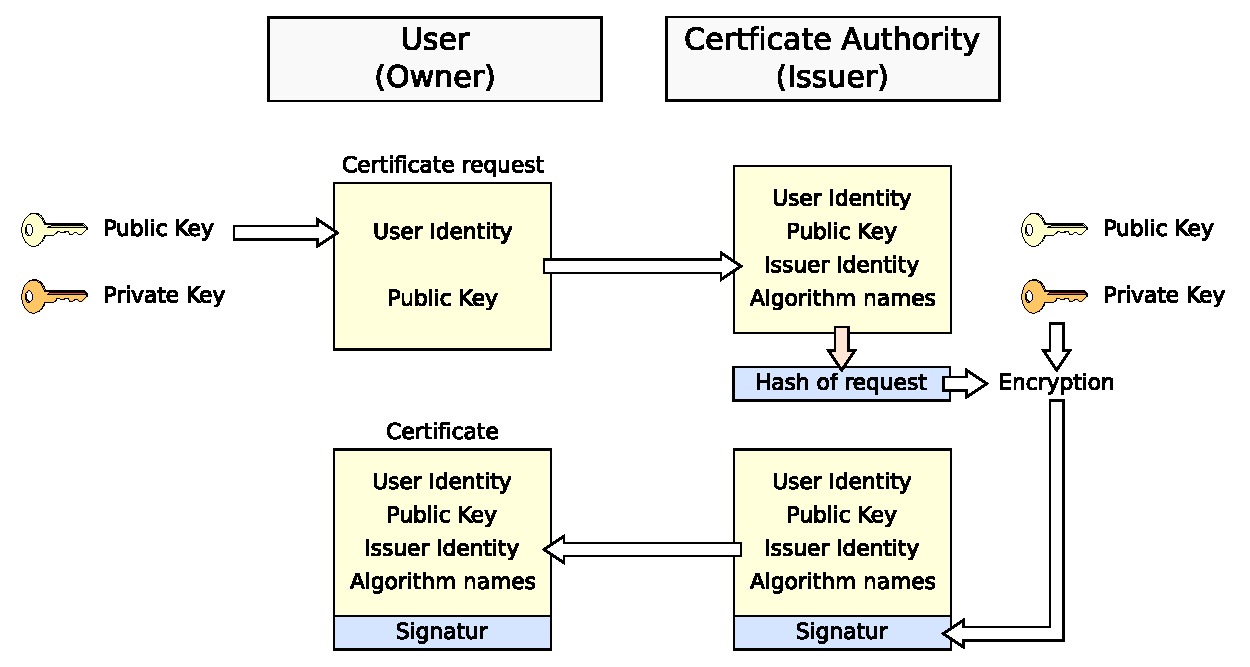
\includegraphics[width=13cm]{tex_tls_echoservice/certificates.pdf}
	\mycaption{Procedure of certificate signing.}{}
	\label{fig:certificate_request}
\end{figure}
In the first step, a private and a public key will be generated by the requester.
The public key together with a textual description of the identity depict the request which will be transmitted to a CA.
After the CA successfully verified the validity of the request, the identity of the CA and the name of the used encryption algorithms are added.
The collected data will represent the plain text of the certificate.
In order to ensure the integrity of the text, a hash value will be created.
This is a fixed-sized short string which is generated by an algorithm based on an arbitrary long given text.
The algorithm is designed such that a small change in the text will cause the hash value to change almost like a random function.
Thus, the hash value can be used a fingerprint of the text.
The CA signs the plain certificate by encrypting its hash value with its private key.
Finally the signed certifcate will be returned to the requester.
If an outside person wants to verify the certificate owner, the encrypted hash value has to be decrypted by the public key of the CA and a hash value has to be created with the same algorithm in order to compare them.\\


Figure~\ref{fig:verification_of_certificates} shows a usecase in which Alice wants to resolve the identity of Bob.
Alice submits her request to Bob along with a challange consisting of a random number $n$. 
Bob encrypts the number with his private key and returns it together with his certificate.
The random number ensures that it is not possible to repeat a message (integrity) and to prove that the communication partner holds the private key.
Alice uses the public key of Bob to decrypt the challenge. 
If the decrypted number is equal to the transmitted number, Alice can reason that the identity of Bob is to be trusted in case she is trusting the CA which has signed Bobs certificate.\\

In the given example, Alice only trusts the CA 2 but not CA 1.
To resolve the identity of CA 1, Alice establishes a connection to CA 1 and submits another random number $n$ as a challenge.
The CA 1 encrypts the challenge with its private key and sends the result along with its certificate back to Alice. 
Alice successfully compares the returned number. Additionally she validates the certificate of CA 1 with the pre-configured certificate of CA 2..
Since the certificate was signed by CA 2 which is pre-configured to be trusted, she also trusts CA 1 and in conclusion the identity of B.
In summary, Alice knows she is talking to Bob.
If Bob also wants to be sure who he's talking to, then the same procedure has to be done to confirm the identity of Alice.
The TLS mode in which both endpoints are ensuring themselves to whom they are talking to is called \textit{bilateral connection mode}.\\


When the client is aware of the server's authentity, the confidential treatment of its data is guaranteed such that one can be sure the data won't be revealed to a third party (server-sided confidentiality). 
On the other side, if the server is aware of the client authentity, the access to services and resources can be controlled (access control). Thus, in case of services, the results will only be passed back to the right person (client-sided confidentiality). 
As one can see confidentiality, authentication, integrity and non-repudiation are now established.\\

\begin{figure}[tbh]
	\centering%epstopdf verification.eps 
	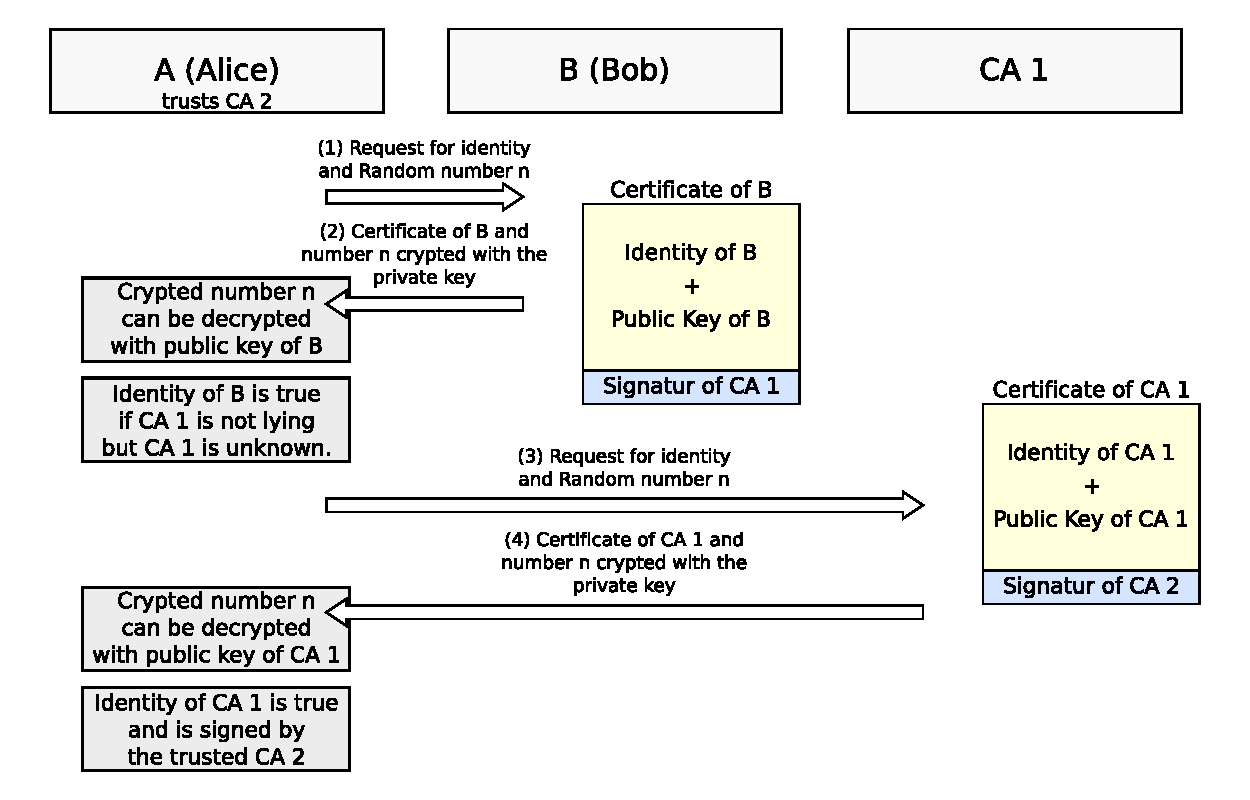
\includegraphics[width=13cm]{tex_tls_echoservice/verification.pdf}
	\mycaption{Usecase in which Alice resolves the identity of Bob.}{In order to resolve the identity of Bob, Alice sends a request for Bob's identity along with a newly created random number to Bob. Bob encrypts the received number using his private key and returns his public key to Alice. Due to the random number can only be encrypted by the owner of the private key, Alice is able ot verify that the certificate was transmitted by his owner. Since the certificate was signed by the CA 1, which she is not per-configured to be trust, Alice needs to resolve also the identity of CA 1. The request is done in the same manner, but this time the certificate is signed by the trusted CA 2. Due to the fact she is now able to trust CA 1, Alice can now also trust the identity of Bob.}
	\label{fig:verification_of_certificates}
\end{figure}

Certificates have several advantages.
They are scaling very good with the amount of users because CAs can create new sub-CAs such that the load is balanced (certificates of a CA may be cached).
Furthermore, no critical information is exchanged for the establishment of a connection (in particular: no secret key is shared which may get intercepted).
Instead, a set of pre-configured CAs which will be in general provided by the operation system is needed.
In respect of ARC it is obvious that the access to the grid shall be under the control of its administrator.
To do so, the administrators have to create their own CAs which are in charge of creating certificates for new users.
The identity of the created CA has to be added to the directory of pre-configured CAs.
Many universities have prepared local certificate authorities. And every user can establish his own. Certificates in general, however, have found entry to regular computer users, for instance with the FernUniversity Hagen (https://ca.fernuni-hagen.de/) who use that technology for their remote students to hand in exercises.\\


A CA which controls access to a grid can be considered as a virtual organsiation (VO).
It may involve organisations close to the leading organisation as well as structure which are not formally associated with it.
In most cases the basic idea is to share ressources. \task{this para will need some overhaul - SM; jup, that a bit short... unfortunatly I am not very familiar with that stuff, but I am on it :-( - MG}

\clearpage
\section{Service}


In order to create a secure connection we hence need two certificates: a client certificate and a service certificate.
The CA of the certificate has to be pre-configured on the counterpart and furthermore, the owner of the certificate has to hold the fitting private key.
For the given example X.509-certificates in the PEM format will be used which are standardised by the ITU-T.
Altogether six files are needed:\\
\\
\begin{tabular}{l@{~---~}p{13cm}}
\textbf{clientCA}   & The CA which guarantees for the identity of the client \\
\textbf{clientCERT} & The certificate of the client. \\
\textbf{clientKEY}  & The private key of the client (should be kept in safe custody).\vspace{2ex}\\
\textbf{serverCA}   & The CA which guarantees for the identity of the server \\
\textbf{serverCERT} & The certificate of the server. \\
\textbf{serverKEY}  & The private key of the server (should be kept in safe custody).\\
\end{tabular}
\forcelinebreak
\\






To get this service running, the six files have to be distributed. The server should hold the files: serverCERT.pem, serverKEY.pem and clientCA.pem. The client on the other side should own the files: clientCERT.pem, clientKEY.pem and serverCA.pem.
Within the source code directory that accompanies this document certificates with corresponding names are prepared. Due to certificates have a limited period of validity, these certificates may no longer be accepted by the communication parter.
One has to create new certificates to ensure the proper work of the TLS Web Service.\\


Several tools are available which allow the handling for more advanced UNIX users. In order to create a first basic set of certificates signed by a self created CA, the shell scripts \textit{createMasterCA.sh} and \textit{createSlaveCert.sh} can  be found within the directory \textit{src/services/tlsechoservice/certFactory} may be used. The script \textit{createMasterCA.sh} will create a new CA and will overwrite older ones. The script \textit{createSlaveCert.sh} creates several certificates signed by the CA.\\


The TLS Echo Web Service implementation is almost the same as the one presented in the previous chapter. Merely the Class name and the namespace of the service have been changed. The only modification is done within the server configuration file which is displayed in Listing~\ref{lst:tls_echo_arched_xml}.
\lstsetARCHEDXML
\lstinputlisting
	[
	label=lst:tls_echo_arched_xml,float=htb,
	caption={[HED configuration file for the Arc intern echo service. Filename: arcecho\_no\_ssl.xml]
	\textbf{HED configuration file for the Arc intern echo service. Filename: arcecho\_no\_ssl.xml\textcolor{white}{hmf}}}
	]
{../examples/src/services/tlsechoservice/arched_tls_echoservice.xml}
The first change is in line~\ref{lst_code:tls_echo_arched_xml_plugin}. As to be seen, another plugin called \textit{mcctls} will be loaded by the \textit{ModuleManager}. The second change is the new element which has been placed between the TCP and the HTTP component, see line~\ref{lst_code:tls_echo_arched_xml_component}. Within the TLS element the certificates can be declared using the elements \textit{KeyPath}, \textit{CertificatePath}, \textit{CACertificatePath} and \textit{CACertificatesDir}.
% \begin{verbatim}
% <KeyPath>./clientKey.pem</KeyPath>
% 
% <CertificatePath>./clientCert.pem</CertificatePath>
% 
% <CACertificatePath>./serviceCA.pem</CACertificatePath>
% 
% <CACertificatesDir>/etc/grid-security/certificates</CACertificatesDir>
% \end{verbatim}
% or
% \begin{verbatim}
% <ClientSSLConfig FromFile='filename'/>
% \end{verbatim}
% \task{You can put the ClientSSLConfig into a separate file, then use <ClientSSLConfig FromFile='filename'/> in each service, and then you don't need to change everywhere - proposed by Zsombor - but I can't find any example *hrmlgrmpf*...}


%\lstsetCPP
%\lstinputlisting
%	[
%	label=lst:tls_echo_service_cpp,
%	caption={[HED configuration file for the Arc intern echo service. Filename: arcecho\_no\_ssl.xml]
%	\textbf{HED configuration file for the Arc intern echo service. Filename: arcecho\_no\_ssl.xml\textcolor{white}{hmf}}}
%	]
%{../examples/src/services/tlsechoservice/tlsechoservice.cpp}
%
% Lassen wir mal weg....
%
%
% \lstsetKSH
% \begin{lstlisting}[
% label=lst:tls_echo_arched_invoke,float=htb,
% caption={[Transformation in eine uniforme konzentrische Verteilung.]
%          \textbf{Transformation in eine uniforme konzentrische Verteilung.\textcolor{white}{hmf}}}]
% $ rm -f /var/log/arc/arched.log
% $ arched -c arched_echoservice.xml  && echo jo ||echo n
% $ tail -n100 -f /var/log/arc/arched.log
% $ killall arched
% \end{lstlisting}
% 
%        ...das auch.....


\clearpage
\section{Client}

In this section a new way to implement the client will be introduced. As already mentioned in section~\ref{sec:timeservice_client}, the protocol stack of the client is built up in almost the same way as the one of the service. Indeed, the class~\textit{ClientSOAP} composes the stack with the same MCCs used for the service. Once this is known, it is self-evident to create the client in a simlar manner like the service with an own configuration file.
Listing~\ref{lst:tls_echo_client_cpp} shows the source code of the client program. The main difference to the simple Echo Client presented in the previous chapter is that now the information about the client protocol stack is encapsulated within a configuration file.\\
\lstsetCPP
\lstinputlisting
	[
	label=lst:tls_echo_client_cpp,
	caption={[Client programm which is capable to load a configuration file]
	\textbf{Client programm which is capable to load a configuration file}}
	]
{../examples/src/clients/tlsechoclient/tlsechoclient.cpp}


The file containing the client configuration is specified within the command line. 
Its content will be loaded in the code fragment starting at line~\ref{lst_code:tls_echo_client_cpp_getfilecontent}. 
Later, in line~\ref{lst_code:tls_echo_client_cpp_loadconfiguration}, the configuration will be parsed into XML and than transfered into a chain of components which is wrapped by the object \textit{loader}. In order to process a message, an entry point within the chain has to be disclosed. To implement a SOAP client, we are looking for the SOAP component. 
To get the proper component an operator of MCCLoader is used in line~\ref{lst_code:tls_echo_client_cpp_cliententry}.
The previously used class \textit{ClientSOAP} has eased some workload which now has to be done within the client program.
The payloads now have to be wrapped by message objects which have to be initialised with an \textit{MessageAttribute} object and a \textit{MessageContext} object. After the payload has been wrapped within the message it gets transmitted in almost the same way like before, see lines following by line~\ref{lst_code:tls_echo_client_cpp_createandprocess}. The remainder of the source code is identical to the Echo Client.\\





% Folgender XML Aufruf und Antwort soll \textit{automatisch} generiert werden:






% 
% \lstsetJUSTXML
% \begin{lstlisting}[
% label=lst:tls_echo_request_XML,float=htb,
% caption={[Transformation in eine uniforme konzentrische Verteilung.]
%          \textbf{Transformation in eine uniforme konzentrische Verteilung.\textcolor{white}{hmf}}}]
% <soap-env:Envelope xmlns:tlsecho="urn:tlsecho" xmlns:soap-enc="http://schemas.xmlsoap.org/soap/encoding/" xmlns:soap-env="http://schemas.xmlsoap.org/soap/envelope/" xmlns:xsd="http://www.w3.org/2001/XMLSchema" xmlns:xsi="http://www.w3.org/2001/XMLSchema-instance">
%   <soap-env:Body>
%     <tlsecho:tlsechoRequest>
%       <tlsecho:say operation="ordinary">text_to_be_transmitted</tlsecho:say>
%     </tlsecho:tlsechoRequest>
%   </soap-env:Body>
% </soap-env:Envelope>
% \end{lstlisting}
% 
% 
% 
% 
% 
% 
% \lstsetJUSTXML
% \begin{lstlisting}[
% label=lst:tls_echo_response_XML,float=htb,
% caption={[Transformation in eine uniforme konzentrische Verteilung.]
%          \textbf{Transformation in eine uniforme konzentrische Verteilung.\textcolor{white}{hmf}}}]
% <soap-env:Envelope xmlns:tlsecho="urn:tlsecho" xmlns:soap-enc="http://schemas.xmlsoap.org/soap/encoding/" xmlns:soap-env="http://schemas.xmlsoap.org/soap/envelope/" xmlns:xsd="http://www.w3.org/2001/XMLSchema" xmlns:xsi="http://www.w3.org/2001/XMLSchema-instance">
%   <soap-env:Body>
%     <tlsecho:tlsechoResponse>
%       <tlsecho:hear>[ text_to_be_transmitted ]</tlsecho:hear>
%     </tlsecho:tlsechoResponse>
%   </soap-env:Body>
% </soap-env:Envelope>
% \end{lstlisting}
% 

\chapter{Secure Echo Web Service}

The TLS Echo Web Service, which was presented in the previous chapter, was able to control the access to the HED on a very low layer. 
For the administration of a large VO the kind of security may be too general.
Thus, it is recommended to have a more fine-grained security. 
This chapter discusses how to install a more complex security such that it is possible to limit the access of certain resources to particular users and to constrain their rights on the workstation.\\


The security framework of ARC is based on the same concept of modularity as HED. 
To extend the security of a MCC or a service one only needs to modify the server configuration file. That is done by including a \textit{SecHandler} element into the component or service which contains a PDP element. A small example of a chain component containing a \textit{SecHandler} is shown in Listing~\ref{lst:sec_service_component_xml}. Within the element \textit{Component}, which realises a HTTP layer, an element \textit{SecHandler} is located. It contains three attributes. The  attribute \textit{name} is \textit{arc.authz}, the \textit{event} attribute is \textit{incoming} and the \textit{id} attribute which is \textit{auth}. 
While \textit{id} is only an optional parameter, the attribute \textit{name} causes a certain \textit{SecHandler} to be loaded. %, which again has a certain functionality. 
In case the attribute \textit{name} is assigned to \textit{arc.authz}, the SecHandler provides the functionality of authentication and is able to permit or to deny the access to the next layer. 
Each MCC or Service usually implements two queues of \textit{SecHandlers} --- one for incoming messages and one for outgoing messages. The attribute \textit{event} attaches the present one to the incoming queue. \textit{SecHandlers} are able to intervene the message flow by: manipulating the message content, manipulating the message attributes or to disrupt messages.
Within one component, \textit{SecHandlers} are executed sequentially in the order in which they were attached to the queue. If any of them fails, message processing fails as well~\cite{QIANG_2008}.\\


In order to decide how the \textit{SecHandler} shall modify the message, so called PDP (Policy Decision Point) are used. Within the example a PDP named \textit{simplelist.pdp} is inserted within the \textit{SecHandler} element. The mechanism of this PDP uses a file which contains a list of identities. If the current identity is on the list, the PDP returns a positive result to the \textit{SecHandler}. In general more than one PDP can be defined within one \textit{SecHandler}. The default behaviour in that case is to execute all PDPs sequentially until one fails such that a negativ result will be returned or all return a negativ result such that also a positive result will be passed to the \textit{SecHandler}.\\
%
%
% Weizhong: Verifying, parsing the message attribute, and using the attributes for authorization
%
% Attributes done by: identity.map, delegation.collector
% manipulating content: usernametoken.handler
% disrupt by: arc.authz
\lstsetJUSTXML
\begin{lstlisting}[
label=lst:sec_service_component_xml,float=htb,
caption={[Example of a SecHandler within the component \textit{http.service}.]
         \textbf{Example of a SecHandler within the component \textit{http.service}}}]
<Component name="http.service" id="http">
	<next id="soap">POST</next>
	<SecHandler name="arc.authz" event="incoming" id="auth">
		<PDP name="simplelist.pdp" location="./clientlist.txt"/>
	</SecHandler>
</Component>
\end{lstlisting}




  \begin{table}[htb]
  \centering
  \caption{List of built-in SecHandlers}
  \label{tbl:list_of_sechandler}
  \begin{tabular*}{\textwidth}[t]{p{4cm}p{11cm}}
	\hline
 	\textbf{identity.map}         & Maps the identity of the user to an identity of the workstation.\\
%					realised by a message attribut.\\
 	\textbf{arc.authz}            & Grants access to the next layer.\\
 	\textbf{delegation.collector} & Processes a request for another service located on a different HED.
                                        A certificate, which has a delegation policy embedded, is transfered to the service running that \textit{SecHandler}. Once the has been extracted and verified it will be transfered
                                        to the requested service.
                                        The policy is now available within the HED of the service such that the client is enabled to access the service.\\
                                        % Question how does the client creates the request - with the SecHandler?
 	\textbf{usernametoken.handler}& Generates the WS-Security username-token and adds it into the SOAP header of outgoing
					 messages. In case of incoming messages the SecHandler extracts the WS-Security username-token out of it. The WS-Security standard extends SOAP and describes i.e. how to attach signatures and encryption header to SOAP messages.\\
	\hline
  \end{tabular*}
  \end{table}
% WS-Security describes how to attach signatures and encryption headers to SOAP messages. In addition, it describes how to attach security tokens, including binary security tokens such as X.509 certificates and Kerberos tickets, to messages.
%
  \begin{table}[htb]
  \centering
  \caption{List of built-in PDPs}
\label{tbl:list_of_pdps}
  \begin{tabular*}{\textwidth}[t]{p{4cm}p{11cm}}
	\hline
 	\textbf{allow.pdp}           & Always returns a positive result.\\
	\textbf{deny.pdp}            & Always returns a negative result.\\
 	\textbf{simplelist.pdp}      & Renders a positive result in case the identity corresponds to the listed ones and additionally 
                                       maps the identity to an user of the workstation.\\
 	\textbf{arc.pdp}             & Evaluates the result based on a policy XML file.\\
 	\textbf{delegate.pdp}        & Similar to \textit{arc.pdp} a policy file will be evaluated. But here, the policy document is 
                                       extracted and transfered
                                       by delegation.collector.\\
 	\textbf{pdpservice.invoker}  & Establishes a connection to special service in order to get a policy decision. The PDP service 
                                       implements the same functionality as ARC PDP, except that the evaluation request and 
                                       response is carried by SOAP messages. The benefit of the PDP Service and the PDP Service
                                       Invoker is that the policy evaluation engine can be accessed remotely and maintained centrally.
\\
	\hline
  \end{tabular*}
  \end{table}
%
%
Due to the fact, that presenting all \textit{SecHandlers} and PDPs would go beyond the scope of an introducing tutorial, only a small set of them will be introduced here in detail. 
Nevertheless, the Tables~\ref{tbl:list_of_sechandler} and~\ref{tbl:list_of_pdps} shall give a first overview about existing \textit{SecHandlers} and \textit{PDPs}. For further reading it is recommended to consult the document ``Security framework of ARC1'' written by Weizhong Qiang and Alexandr Konstantinov. The present chapter is closly related to it.\\


The Secure Echo Web Service which will be presented in this chapter, is using the \textit{SecHandlers}: \textit{indentity.map} and \textit{arc.authz}, and the \textit{PDPs}: \textit{allow.pdp}, \textit{simplelist.pdp} and \textit{arc.pdp}. \\


\section{Service}

Listing~\ref{lst:sececho_service_cpp} contains the source code of the Secure Echo Web Service. As one can see, the only difference, compared to the source code of the previous section, is the additional code to process the \textit{SecHandler} starting at line~\ref{lst_code:sececho_service_cpp_process_secH}. Obviously only the incoming queue is processed and in case the \textit{SecHandler} fails, the SOAP service returns a fault message. The file, which is revealing a lot more information, is the server configuration file which is shown in Listing~\ref{lst:sececho_server_configuration_file_xml}. 
To enable \textit{SecHandlers} to work with identities, it is almost essential to utilise the TLS layer.
% Fixed IP are also possible but not recommended..
The TLS layer extracts the identity such that it later can be used to process the \textit{SecHandler}.
In line~\ref{lst_code:arched_sec_conffile_plugins} and line~\ref{lst_code:arched_sec_conffile_plugins2} two additional plugins 
are named to be loaded which are implementing of the \textit{SecHandlers} and \textit{PDPs}.
%
%  FIRST ONE
%
The first \textit{SecHandler} is declared at line~\ref{lst_code:arched_sec_conffile_secH2}. 
The PDP \textit{allow.pdp} always returns a positive result, such that everyone who passes the \textit{SecHandler} is mapped to the user \textit{nobody}. 
%
% SECOND ONE
%
The second \textit{SecHandler} limits the access to the SOAP services using the \textit{arc.authz} \textit{SecHandler} and the \textit{simplelist} policy, see line~\ref{lst_code:arched_sec_conffile_secH1}. A similar example was already shown in Listing~\ref{lst:sec_service_component_xml}. The \textit{simplelist} policy returns a positive result if the identity of the certificate corresponds to an identity within the file \textit{clientlist.txt}. A small example of such a file is displayed in Listing~\ref{lst:simplelist_example}.
\lstsetCPP
\lstinputlisting
	[
	label=lst:sececho_service_cpp,
	caption={[Source code of the Secure Echo Service.]
	\textbf{Source code of the Secure Echo Service.}}
	]
{../examples/src/services/secechoservice/secechoservice.cpp}
%
%
The first part of an entry needs to be the distinguished name (DN) of the current client. A DN is a string which represents a user uniquely and is created using the identity of the certificate. To get the correct DN of a client one can use the TLS Echo Web Service and check the log-file. The second part of an entry specifies the user the identity shall be mapped to. In the present case, the identity will be mapped to \textit{griduser}. In case the policy is unable to match the identity, the PDP returns a negativ result.
The \textit{SecHandler} within the SOAP component limits the access of SOAP to a certain group of users.
%
%
% The third ONE
The last \textit{SecHandler}, used in the server configuration file, is to be seen starting with line~\ref{lst_code:arched_sec_conffile_secH3}. The \textit{SecHandler} is chosen to be \textit{arc.authz} which leads to the fact that the access to the Echo Web Service will be limited one more time to a subset of the group. The policy \textit{arc.pdp} returns a positive result in case the rules encapsulated within the file \textit{policy.xml} will return a positive result.\\
\lstsetARCHEDXML
\lstinputlisting
	[
	label=lst:sececho_server_configuration_file_xml, float=htb
	caption={[HED configuration file for the Arc intern echo service. Filename: arcecho\_no\_ssl.xml]
	\textbf{HED configuration file for the Arc intern echo service. Filename: arcecho\_no\_ssl.xml\textcolor{white}{hmf}}}
	]
{../examples/src/services/secechoservice/arched_sec_echoservice.xml}



\lstsetKSH
\begin{lstlisting}[
label=lst:simplelist_example, float=htb,
caption={[Appearence of the file used by \textit{simplelist.pdp}.]
         \textbf{Appearence of the file used by \textit{simplelist.pdp}.}}]
$ cat clientlist.txt
"/C=US/S=Maine/OU=Literary character/O=Ka-Tet Corp./CN=Roland Deschain" griduser
"/C=US/S=Maine/OU=Literary character/O=Ka-Tet Corp./CN=Susannah Dean" griduser
$
\end{lstlisting}

If the PDP \textit{arc.authz} is used, a bunch of requests will be generated for the client. The requests are compared with the rules defined in the policy and for each rule a decision is made.
A sample policy is shown in Listing~\ref{lst:sececho_policy_xml}. The main element is \textit{policy} which encloses three elements called \textit{Rule}\footnote{The latest XML schema for defining an \textit{arc.pdp} policy can be found at \url{http://svn.nordugrid.org/trac/nordugrid/browser/arc1/trunk/src/hed/shc/arcpdp/Policy.xsd}}. 
Two types of rules are possible: a permitting or a denying rule.
A Rule may have four different decision states:
\begin{itemize}
 \item PERMIT --- A permitting rule returns the decision permit if one request fits to the rule and 
the request is fullfilled by the rule. (A denying rule would return deny in that case)
 \item DENY --- A permitting rule returns the decision deny if one request fits to the rule  and the request is not fullfilled by the rule. (A denying rule would return permit that case)
 \item INDETERMINATE --- Requests and rule have some parts which not fits
(i.e. shibboleth identity is checked, but user has identified himself via X.509 and additionally an existing resource is requested)
 \item NOT\_APPLICABLE --- If the request doesn't fit with the rule at all. (i.e. if the 
request is for the HTTP method GET, but the rule checks the method POST)
\end{itemize}
\forcelinebreak

Once all rules are evaluated, a decision for the policy has to be generated which will depend on the results of the rules.
The policy element attribute \textit{CombiningAlg} determines how the final result will be generated. Two possibilities are given:
\begin{itemize}
 \item \textbf{Deny-Overrides} (default) 
 \begin{itemize}
	\item If there is at least one DENY in results final result is DENY. 
	\item Otherwise if there is at least one PERMIT, the final result is PERMIT.
	\item Otherwise if there is at least one NOT\_APPLICABLE final result is NOT\_APPLICABLE.
	\item Otherwise final result is INDETERMINATE.
 \end{itemize}
  \item \textbf{Permit-Overrides}
 \begin{itemize}
 	\item If there is at least one PERMIT in results final result is PERMIT.
 	\item Otherwise if there is at least one DENY the final result is DENY.
 	\item Otherwise if there is at least one NOT\_APPLICABLE final result is NOT\_APPLICABLE.
 	\item Otherwise final result is INDETERMINATE.
 \end{itemize}
\end{itemize}
\forcelinebreak

A rule is devided into four sub-elements: \textit{Subjects}, \textit{Resources}, \textit{Actions} and \textit{Conditions}. 
The element \textit{Subjects} defines who shall be affected by that rule.
The identities can be specified using the DN of the certificate.
The second element determines the \textit{Resources} which shall be examined by the rule (i.e. using a certain HTTP path).
The \textit{Actions} are specifing the intended usage of the resource the rule shall survey.
The last element \textit{Condition} defines somewhat like Time, Duration, namespace of a SOAP message etc. which are needed to be fulfilled. The detailed description of these conditions is rather extensive and beyond the scope of this tutorial. Please refer to the further going tutorials which are listed in the appendix of this tutorial.\\


Within the sample policy, which was shown in Listing~\ref{lst:sececho_policy_xml}, three different examples of rule states are prepared: PERMIT, INDETERMINATE and NOT APPLICABLE.
The first rule, starting at line~\ref{lst_code:policy.xml_rule1}, is fitting to the server configuration file such that a user with a suitable identity will produce the state PERMIT. 
Since there is no rule within the policy which will have the DENY state, in particular no rule that could have matched earlier, this rule lets the client pass the PDP.
The second rule begins after line~\ref{lst_code:policy.xml_rule2}. It is arranged in a manner such that the state INDETERMINATE will be induced. Two things are checked within it: the identity based on authentication method Shibboleth\footnote{Shibboleth is an open-source implementation for authentication and authorization based on the XML standard SAML (Security Assertion Markup Language).} 
and the path of the requested HTTP URL. Due to the fact, that the HTTP path is fitting to the requested one, but the authentication was not done by Shibboleth, the rule is not able to decide for a DENY or a PERMIT state --- the rule produces an INDETERMINATE state.
The last rule is defined in line~\ref{lst_code:policy.xml_rule3}. It is constructed such that is permits the access to the HTTP method GET. 
One can see, that within the server configuration file the Web Service uses the method POST. If a client wants to access the Service and reaches the PDP, a couple of requests are generated which are describing the manner the client wants to access the serivice. Some of these request will concern the HTTP method GET. In these cases, the rule returns NOT APPLICABLE. In the cases where the requests for a HTTP method is missing (i.e. in the request which only concerns the SOAP access) the state of the rule will be INDETERMINATE.\\
\lstsetJUSTXML
\lstinputlisting
	[
	label=lst:sececho_policy_xml, float=htb,
	caption={[Policy file for the \textit{arc.pdp} policy decision point.]
	\textbf{Policy file for the \textit{arc.pdp} policy decision point.}}
	]
{../examples/src/services/secechoservice/policy_example.xml}


To get an impression in how the requests look like, one can check the log-file (the log level needs to be set to DEBUG).


\section{Client}

The security introduced to the server has no effect on the client, such that the source code is completely identical. Even the client configuration file doesn't need to be changed.

















 
\chapter{Persistent Webservice}


export ARC\_BARTENDER\_URL
\chapter{Appendix}

\section{Useful tutorials and documentations}

In order to learn more about ARC several other tutorials and documentations have been written:
\begin{itemize}
 \item ARC Web Services Quick Usage Guide~\cite{2008_UNKNOWN}
 \item The Hosting Environment of the Advanced Resource Connector middleware~\cite{2008_Cameron}.
 \item Security framework of ARC1~\cite{QIANG_2008}.
 \item Documentation of the ARC storage system~\cite{Nagy_2008}.
 \item Eclipse WTP 1.5.1, Introduction to the WSDL Editor, \url{http://wiki.eclipse.org/index.php/Introduction_to_the_WSDL_Editor}


\end{itemize}




\section{Important XSD files}\label{sec:impXSD}

\lstsetJUSTXML
\lstinputlisting
	[
	label=lst:mcc.xsd,
	caption={[XML schema of configuration files.]\textbf{XML schema of configuration files.}}
	]{../../../src/hed/libs/loader/mcc.xsd}

\lstsetJUSTXML
\lstinputlisting
	[
	label=lst:tcp.xsd,
	caption={[XML schema of the TCP component.]\textbf{XML schema of the TCP component.}}
	]{../../../src/hed/mcc/tcp/tcp.xsd}

\lstsetJUSTXML
\lstinputlisting
	[
	label=lst:tls.xssd,
	caption={[XML schema of the TLS component.]\textbf{XML schema of  the TLS component.}}
	]{../../../src/hed/mcc/tls/tls.xsd}

\lstsetJUSTXML
\lstinputlisting
	[
	label=lst:http_xsd,
	caption={[XML schema of the HTTP component.]\textbf{XML schema of the HTTP component.}}
	]{../../../src/hed/mcc/http/http.xsd}









% 
% Questions:
% \begin{itemize}
%  \item The images of the HED structure always are ordered like: TCP - TLS - HTTP - PLEXER - SOAP - Web Service   but the source code examples are: TCP - TLS - HTTP - SOAP - PLEXER - Web Service\\
% --- ANSWER BY WEIZHONG: In my understanding (because plexer is not my initial idea), plexer (as a sort of hub) can be put at both after http or soap. If you put after soap,then you are doing switching for different web services. While I put it after http, because somehow, I need to switch the message after http-processing, in more detail, one branch for soap and then web service/s,
%  one branch for a non-soap service/server (the SP Service is not a service based on SOAP, actually it is based on http, so it is kind of web application).
% 
% \item The HED does not act as a front end server which delegates its task to new instances acting on a diffrent port such that the daemon is always available. 
% \end{itemize}

% 
% 
 \task{RENAMING HED configuration file into~ARC service configuration file - proposed by Marek}
 \task{(echo service) client configuration file - proposed by Marek}
 \task{Check commas using \url{http://leo.stcloudstate.edu/punct/comma.html}}

 \task{Bisher noch nicht beachtet: \\
\\\textcolor{urgent}{
In general, a comma is used when the
subordinate clause precedes the main clause, like this:\\
\\
``When subjects were aware of the purpose of the experiment, no effect was
observed.''\\
\\
Furthermore:\\
\\
      ``We discarded specimens that had become contaminated.''\\
\\
In this case, the relative clause is restrictive because it defines exactly which specimens
were discarded. Restrictive clauses should not be preceded by a comma.\\
\\
  In contrast, a non-restrictive clause gives additional information about an object that
has already been identified; for example:\\
\\
      ``The file server uses the XFS file system, which supports journaling and pro-
      vides excellent performance.''\\
\\
In this case, the relative clause does not restrict or define the particular file system being
talked about, but merely provides additional information. Non-restrictive clauses should
be preceded by a comma.}}





\bibliography{literature}
\bibliographystyle{IEEEtran}                       % A nice bibliography style


\end{document}
